\documentclass{article}
\usepackage{fullpage}
\usepackage[utf8]{inputenc}
\usepackage{pict2e}
\usepackage{amsmath}
\usepackage{enumitem}
\usepackage{eurosym}
\usepackage{mathtools}
\usepackage{amssymb, amsfonts, latexsym, cancel}
\setlength{\parskip}{0.3cm}
\usepackage{graphicx}
\usepackage{fontenc}
\usepackage{slashbox}
\usepackage{setspace}
\usepackage{gensymb}
\usepackage{accents}
\usepackage{adjustbox}
\setstretch{1.35}
\usepackage{bold-extra}
\usepackage[document]{ragged2e}
\usepackage{subcaption}
\usepackage{tcolorbox}
\usepackage{xcolor, colortbl}
\usepackage{wrapfig}
\usepackage{empheq}
\usepackage{array}
\usepackage{parskip}
\usepackage{arydshln}
\graphicspath{ {images/} }
\renewcommand*\contentsname{\color{black}Índice} 
\usepackage{array, multirow, multicol}
\definecolor{lightblue}{HTML}{007AFF}
\usepackage{color}
\usepackage{etoolbox}
\usepackage{listings}
\usepackage{mdframed}
\setlength{\parindent}{0pt}
\usepackage{underscore}
\usepackage{hyperref}
\usepackage{tikz}
\usepackage{tikz-cd}
\usetikzlibrary{shapes, positioning, patterns}
\usepackage{tikz-qtree}
\usepackage{biblatex}
\usepackage{pdfpages}
\usepackage{pgfplots}
\usepackage{pgfkeys}
\addbibresource{biblatex-examples.bib}
\usepackage[a4paper, left=1cm, right=1cm, top=1cm,
bottom=1.5cm]{geometry}
\usepackage{titlesec}
\usepackage{titletoc}
\usepackage{tikz-3dplot}
\usepackage{kbordermatrix}
\usetikzlibrary{decorations.pathreplacing}
\newcommand{\Ej}{\textcolor{lightblue}{\underline{Ejemplo}}}
\setlength{\fboxrule}{1.5pt}

% Configura el formato de las secciones utilizando titlesec
\titleformat{\section}
{\color{red}\normalfont\LARGE\bfseries}
{Tema \thesection:}
{10 pt}
{}

% Ajusta el formato de las entradas de la tabla de contenidos
\addtocontents{toc}{\protect\setcounter{tocdepth}{4}}
\addtocontents{toc}{\color{black}}

\titleformat{\subsection}
{\normalfont\Large\bfseries\color{red}}{\thesubsection)}{1em}{\color{lightblue}}

\titleformat{\subsubsection}
{\normalfont\large\bfseries\color{red}}{\thesubsubsection)}{1em}{\color{lightblue}}

\newcommand{\bboxed}[1]{\fcolorbox{lightblue}{lightblue!10}{$#1$}}
\newcommand{\rboxed}[1]{\fcolorbox{red}{red!10}{$#1$}}

\DeclareMathOperator{\N}{\mathbb{N}}
\DeclareMathOperator{\Z}{\mathbb{Z}}
\DeclareMathOperator{\R}{\mathbb{R}}
\DeclareMathOperator{\Q}{\mathbb{Q}}
\DeclareMathOperator{\K}{\mathbb{K}}
\DeclareMathOperator{\im}{\imath}
\DeclareMathOperator{\jm}{\jmath}
\DeclareMathOperator{\col}{\mathrm{Col}}
\DeclareMathOperator{\fil}{\mathrm{Fil}}
\DeclareMathOperator{\rg}{\mathrm{rg}}
\DeclareMathOperator{\nuc}{\mathrm{nuc}}
\DeclareMathOperator{\dimf}{\mathrm{dimFil}}
\DeclareMathOperator{\dimc}{\mathrm{dimCol}}
\DeclareMathOperator{\dimn}{\mathrm{dimnuc}}
\DeclareMathOperator{\dimr}{\mathrm{dimrg}}
\DeclareMathOperator{\dom}{\mathrm{Dom}}
\DeclareMathOperator{\infi}{\int_{-\infty}^{+\infty}}
\newcommand{\dint}[2]{\int_{#1}^{#2}}

\newcommand{\bu}[1]{\textcolor{lightblue}{\underline{#1}}}
\newcommand{\lb}[1]{\textcolor{lightblue}{#1}}
\newcommand{\db}[1]{\textcolor{blue}{#1}}
\newcommand{\rc}[1]{\textcolor{red}{#1}}
\newcommand{\tr}{^\intercal}

\renewcommand{\CancelColor}{\color{lightblue}}

\newcommand{\dx}{\:\mathrm{d}x}
\newcommand{\dt}{\:\mathrm{d}t}
\newcommand{\dy}{\:\mathrm{d}y}
\newcommand{\dz}{\:\mathrm{d}z}
\newcommand{\dth}{\:\mathrm{d}\theta}
\newcommand{\dr}{\:\mathrm{d}\rho}
\newcommand{\du}{\:\mathrm{d}u}
\newcommand{\dv}{\:\mathrm{d}v}
\newcommand{\tozero}[1]{\cancelto{0}{#1}}
\newcommand{\lbb}[2]{\textcolor{lightblue}{\underbracket[1pt]{\textcolor{black}{#1}}_{#2}}}
\newcommand{\dbb}[2]{\textcolor{blue}{\underbracket[1pt]{\textcolor{black}{#1}}_{#2}}}
\newcommand{\rub}[2]{\textcolor{red}{\underbracket[1pt]{\textcolor{black}{#1}}_{#2}}}

\author{Francisco Javier Mercader Martínez}
\date{}
\title{Señales y Sistemas\\Problemas Tema 1: Conceptos Básicos de Señales y Sistemas}

\begin{document}
\maketitle
\begin{enumerate}[label=\color{red}\textbf{\arabic*)}]
  \item \lb{Exprese cada uno de los siguientes números complejos en su parte real e imaginaria $(a+jb)$:}
    \begin{multicols}{2}
    \begin{itemize}[label=\color{red}\textbullet, leftmargin=*]
      \item $\lb{\dfrac{1}{2}e^{j\pi} =}\dfrac{1}{2}(\cos(\pi)+j\sin(\pi))=-\dfrac{1}{2}$
      \item $\lb{\dfrac{1}{2}e^{-j\pi} =}\dfrac{1}{2}(\cos(\pi)-j\sin(\pi))=-\dfrac{1}{2}$ 
      \item $\lb{e^{j\frac{\pi}{2} }=} \cos\left( \dfrac{\pi}{2} \right) +j\cdot \sin\left( \dfrac{\pi}{2} \right) =j$ 
      \item $\lb{e^{-j\frac{\pi}{2} } =} \cos\left( \dfrac{\pi}{2} \right) -j\cdot \sin\left( \dfrac{\pi}{2} \right) =-j$ 
      \item $\lb{e^{j\frac{5\pi}{2} } =} \cos\left( \dfrac{5\pi}{2} \right) +j\cdot \sin\left( \dfrac{5\pi}{2} \right) =j$ 
      \item $\lb{\sqrt{2} e^{j\frac{\pi}{4} } =}\sqrt{2}\cdot \left(\cos\left( \dfrac{\pi}{4} \right) +j\cdot \sin\left( \dfrac{\pi}{4} \right)\right) =1+j$ 
      \item $\lb{\sqrt{2} e^{j\frac{9\pi}{4} } =} \sqrt{2}\cdot  \left(\cos\left( \dfrac{9\pi}{4} \right) +j\cdot \sin\left( \dfrac{9\pi}{4} \right) \right)=1+j$ 
      \item $\lb{\sqrt{2} e^{-j\frac{9\pi}{4} } =} \sqrt{2}\cdot  \left(\cos\left( \dfrac{9\pi}{4} \right) -j\cdot \sin\left( \dfrac{9\pi}{4} \right)\right) =1-j$ 
      \item $\lb{\sqrt{2} e^{-j\frac{\pi}{4} } =} \sqrt{2}\cdot  \left(\cos\left( \dfrac{\pi}{4} \right) -j\cdot \sin\left( \dfrac{\pi}{4} \right)\right) =1-j$
    \end{itemize}
  \end{multicols}
  \item \lb{Exprese cada uno de los siguientes números complejos en su módulo y fase ($|z|e^{j\varphi(z)}$ con $\varphi(z)\in [-\pi,\pi]$):} 
      \begin{itemize}[label=\color{red}\textbullet, leftmargin=*]
        \item $\lb{5:}\begin{cases}
          |z|=\sqrt{5^2+0^2} =5\\
          \varphi=\arctan\left( \dfrac{0}{5} \right) =0
        \end{cases}\longrightarrow 5 $ 
        \item $\lb{-2:}\begin{cases}
          |z|=\sqrt{(-2)^2+0^2}=2\\
          \varphi=\arctan\left( \dfrac{0}{-2} \right) =\pi
        \end{cases} \longrightarrow 2e^{j\pi} $ 
        \item $\lb{-3j:} \begin{cases}
          |z|=\sqrt{0^2+(-3)^2}=3\\
          \varphi=\arctan\left( \dfrac{-3}{0} \right) =-\dfrac{\pi}{2}
        \end{cases}\longrightarrow 3e^{-j\frac{\pi}{2} } $ 
        \item $\lb{-j \dfrac{\sqrt{3} }{2}:} \begin{cases}
          |z|=\sqrt{0^2+\left( -\dfrac{\sqrt{3} }{2} \right) ^2}=\dfrac{\sqrt{3} }{2}\\
          \varphi=\arctan\left( \dfrac{-\frac{\sqrt{3} }{2} }{0} \right) =-\dfrac{\pi}{2}
        \end{cases}\longrightarrow \dfrac{\sqrt{3} }{2}e^{-j\frac{\pi}{2} } $ 
        \item $\lb{1+j:} \begin{cases}
          |z|=\sqrt{1^2+1^2}=\sqrt{2}\\
          \varphi=\arctan\left( \dfrac{1}{1} \right) =\dfrac{\pi}{4}
        \end{cases}\longrightarrow \sqrt{2}e^{j\frac{\pi}{4} }  $ 
        \item $\lb{(1-j)^2=-2j:} \begin{cases}
          |z|=\sqrt{0^2+(-2)^2}=2\\
          \varphi=\arctan\left( \dfrac{-2}{0} \right) =-\dfrac{\pi}{2}
        \end{cases}\longrightarrow 2e^{-j\frac{\pi}{2} } $ 
      \item $\lb{j(1-j)=1+j:} \begin{cases}
              |z|=\sqrt{1^2+1^2}=\sqrt{2}\\
              \varphi=\arctan\left( \dfrac{1}{1} \right ) =\dfrac{\pi}{4}
              \end{cases}\longrightarrow \sqrt{2}e^{j\frac{\pi}{4} } $ 
        \item $\lb{\dfrac{1+j}{1-j}=j:} \begin{cases}
          |z|=\sqrt{0^2+1^2}=1\\
          \varphi=\arctan\left(\dfrac{1}{0}\right)=\dfrac{\pi}{2}
        \end{cases}\longrightarrow e^{j\frac{\pi}{2} } $ 
        \item $\lb{\dfrac{\sqrt{2} +j\sqrt{2} }{1+j\sqrt{3} }=\dfrac{\sqrt{6} +\sqrt{2} }{4}+\dfrac{-\sqrt{6} +\sqrt{2} }{4}j:}\begin{cases}
            |z|=\sqrt{\left(  \dfrac{\sqrt{6} +\sqrt{2} }{4}\right)^2+\left( \dfrac{-\sqrt{6} +\sqrt{2} }{4} \right)^2  }=1 \\
          \varphi=\arctan\left( \dfrac{\frac{\sqrt{6}+\sqrt{2}  }{4} }{\frac{-\sqrt{6}+\sqrt{2}  }{4} }  \right) =-\dfrac{1}{12}\pi
        \end{cases}\longrightarrow e^{-j\frac{1}{12} }  $
      \end{itemize}
  \item \lb{Calcule los valores de potencia media y de energía de las siguientes señales:}
    \begin{enumerate}[label=\color{red}\textbf{\alph*)}]
      \item \db{$x(t)=e^{-2t}u(t) $}
        
        \begin{minipage}{0.3\textwidth}
          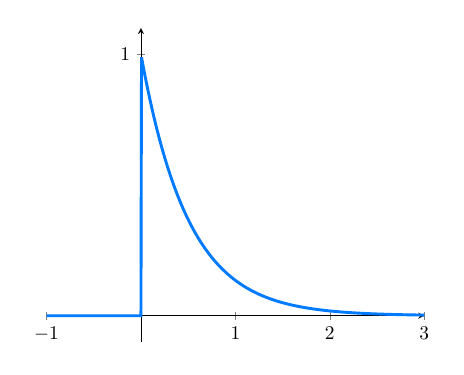
\begin{tikzpicture}[scale=0.7]
          \begin{axis}[
            xmin= -1, xmax= 3,
            ymin= -0.1, ymax = 1.1,
            axis lines = middle,
            ytick={1}, xtick={}
          ]
            \addplot[domain=-2:4, samples=1000, lightblue, line width=1.5]{x<0 ? 0: exp(-2*x)};
          \end{axis}
        \end{tikzpicture}
        \end{minipage} $\begin{array}{l}
          \begin{aligned}
            E_T&= \int_{-\infty}^{\infty} |x(t)|^2\dt=\int_{0}^{\infty} |e^{-2t} |^2\dt=\int_{0}^{\infty} e^{-4t}\dt\\
               &= \left[ -\dfrac{1}{4}e^{-4t}  \right] _0^{\infty}=-\dfrac{1}{4}\cdot [0-1]=\dfrac{1}{4}\mathrm{J} \\
          \end{aligned}\\
          P_m=\lim_{T \to \infty} \dfrac{1}{2T}=\int_{-T}^{T} |x(t)|^2\dt=\lim_{T \to \infty} \dfrac{E_T}{2T}=\dfrac{\frac{1}{4} }{+\infty}=0\mathrm{W} 
        \end{array}$
      \item \db{$x(t)=e^{j\left( 2t+\frac{\pi}{4}  \right) } $} 

        \begin{minipage}{0.3\textwidth}
          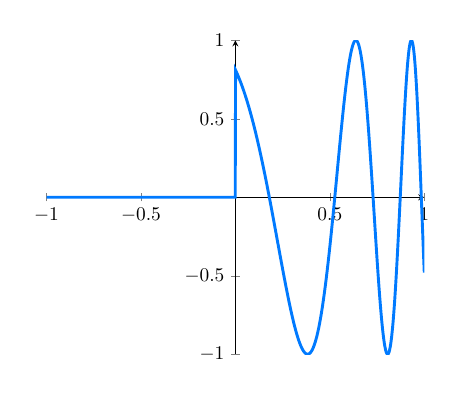
\begin{tikzpicture}[scale=0.7]
          \begin{axis}[
            xmin= -1, xmax= 1,
            ymin= -1, ymax = 1,
            axis lines = middle,
          ]
            \addplot[domain=-1:1, samples=1000, lightblue, line width=1.5]{x<0 ? 0 : sin(deg(exp(2*x+pi/4)))};
          \end{axis}
        \end{tikzpicture}
        \end{minipage}$\begin{aligned}
          E_T&= \int_{-\infty}^{\infty} |x(t)|^2\dt=\int_{-\infty}^{\infty} \left| e^{j\left(2t+\frac{\pi}{4} \right)}  \right|^2\dt    \\
             &= \int_{-\infty}^{\infty} 1^2\dt=[t] _{-\infty}^{\infty}=\infty-(-\infty)=\infty \\
             P_m&= \dfrac{1}{T}\int_{-\frac{T}{2} }^{\frac{T}{2} } \left| e^{j\left( 2t+\frac{\pi}{4}  \right) }  \right| ^2\dt=\dfrac{1}{T}\int_{-\frac{T}{2} }^{\frac{T}{2} } 1\dt   \\
                &= \dfrac{1}{T}\cdot [t]_{-\frac{T}{2} }^{\frac{T}{2} }=\dfrac{1}{T}\cdot \left( \dfrac{T}{2}-\left( -\dfrac{T}{2} \right)  \right) =\dfrac{1}{T}\cdot T=1 \\
        \end{aligned}$
      \item \db{$x(t)=\cos(t)$} 

        \begin{minipage}{0.3\textwidth}
          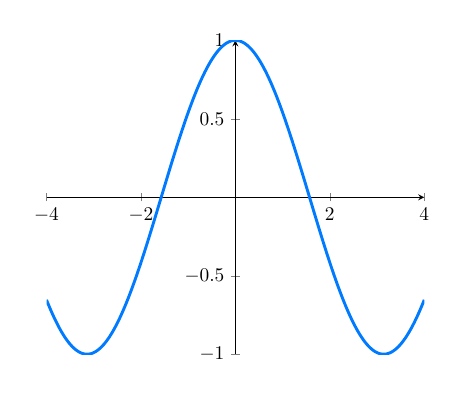
\begin{tikzpicture}[scale=0.7]
          \begin{axis}[
            xmin= -4, xmax= 4,
            ymin= -1, ymax = 1,
            axis lines = middle,
          ]
            \addplot[domain=-4:4, samples=1000, lightblue, line width=1.5]{cos(deg(x))};
          \end{axis}
        \end{tikzpicture}
        \end{minipage}$\begin{aligned}
          E_T&= \int_{-\infty}^{\infty} |x(t)|^2\dt=\int_{-\infty}^{\infty} |\cos(t)|^2\dt=\int_{-\infty}^{\infty} \cos^2(t)\dt    \\
          &= \dfrac{1}{2}\int_{-\infty}^{\infty} 1+\cos(2t)\dt=\dfrac{1}{2}\cdot \left[ t+\dfrac{1}{2}\sin(2t) \right]_{-\infty}^{\infty}   \\
          &=  \\
          P_m&= \dfrac{1}{T}\int_{-\frac{T}{2} }^{\frac{T}{2} } \cos^2(t)\dt=\dfrac{1}{2T}\left[ t+\dfrac{\sin(2t)}{2} \right] _{-\frac{T}{2} }^{\frac{T}{2} }  \\
          &= \dfrac{1}{2T}\left( \dfrac{T}{2}+\dfrac{t}{2}+\dfrac{\sin(T)-\sin(-T)}{2} \right) =\dfrac{1}{2T}\left( T+\tozero{\sin(T)}\:  \right)=\dfrac{1}{2}\mathrm{W}  \\
        \end{aligned}$
      \item \db{$x[n]=\left( \dfrac{1}{2} \right) ^nu[n]$} 

        \begin{minipage}{0.3\textwidth}
          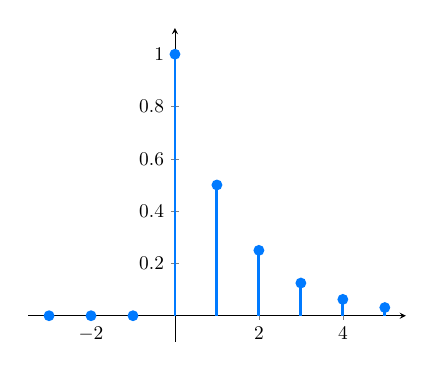
\begin{tikzpicture}[scale=0.7]
          \begin{axis}[
            xmin= -3.5, xmax= 5.5,
            ymin= -0.1, ymax = 1.1,
            axis lines = middle,
          ]
          \addplot[line width=1.5, lightblue, ycomb, mark=*] coordinates {
              (-3,0) (-2,0) (-1,0) (0, 1) (1, 0.5) (2,0.25) (3,0.125) (4, 0.0625) (5, 0.03125)
            };
          \end{axis}
        \end{tikzpicture}
        \end{minipage}$\begin{aligned}
        E_T&= \sum_{n=-\infty}^{\infty} |x[n]|^2=\sum_{n=0}^{\infty} \left| \left( \dfrac{1}{2} \right) ^n \right| ^2=\sum_{n=0}^{\infty} \left( \dfrac{1}{2} \right) ^{2n} \\
        &= \sum_{n=0}^{\infty} \left( \dfrac{1}{4} \right) ^n=\dfrac{1-0\cdot \frac{1}{4} }{1-\frac{1}{4} }=\dfrac{4}{3}\mathrm{J} \\
        P_m&= \lim_{N \to \infty} \dfrac{E_T}{2N+1}=\dfrac{\frac{4}{3} }{+\infty}=0\mathrm{W} \\
        \end{aligned}$
      \item \db{$x[n]=e^{j\left( \frac{\pi}{2} n+\frac{\pi}{8}  \right) } $} 

        \begin{minipage}{0.45\textwidth}
          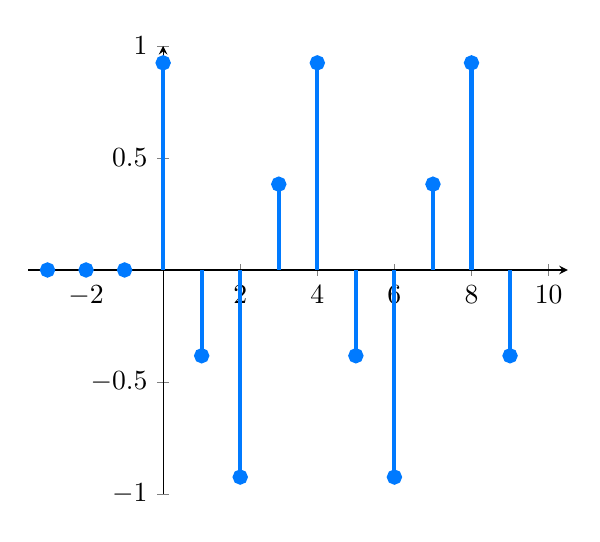
\begin{tikzpicture}
          \begin{axis}[
            xmin= -3.5, xmax= 10.5,
            ymin= -1, ymax = 1,
            axis lines = middle,
          ]
          \addplot[lightblue, line width=1.5, ycomb, mark=*] coordinates {
              (-3, -0.0)
              (-2, -0.0)
              (-1, 0.0)
              (0, 0.9238795325112867)
              (1, -0.3826834323650897)
              (2, -0.9238795325112868)
              (3, 0.38268343236509)
              (4, 0.9238795325112867)
              (5, -0.3826834323650899)
              (6, -0.9238795325112867)
              (7, 0.3826834323650898)
              (8, 0.9238795325112867)
              (9, -0.38268343236508967)
            };
          \end{axis}
        \end{tikzpicture}
        \end{minipage}$\begin{aligned}
        E_T&= \sum_{n=-\infty}^{\infty} |x[n]|^2=\sum_{n=0}^{\infty} \left| e^{j\left( \frac{\pi}{2} n+\frac{\pi}{8}  \right) }  \right| ^2=\sum_{n=0}^{\infty} 1^2=\infty \\
        P_m&= \dfrac{1}{N}\sum_{n=0}^{N-1} |x[n]|^2=\left\{ \omega_0=\dfrac{\pi}{2}\to N=\dfrac{2\pi}{\frac{\pi}{2} }k=4k\underset{k=1}{=} 4\right\}  \\
        &= \dfrac{1}{4}\sum_{n=0}^{3} 1^2=\dfrac{4}{4}=1\mathrm{W} \\
        \end{aligned}$
      \item \db{$x[n]=\cos\left( \dfrac{\pi}{4}n \right)u[n] $} 

        \begin{minipage}{0.45\textwidth}
        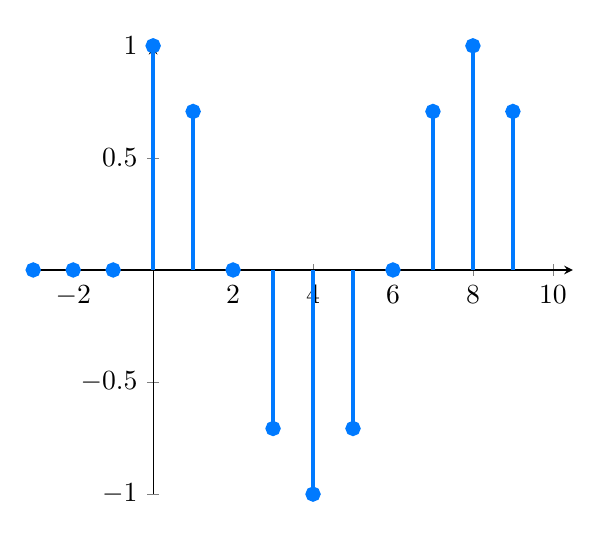
\begin{tikzpicture}
          \begin{axis}[
            xmin= -3, xmax= 10.5,
            ymin= -1, ymax = 1,
            axis lines = middle,
          ]
          \addplot[lightblue, line width=1.5, ycomb, mark=*] coordinates {
              (-3, -0.0)
              (-2, 0.0)
              (-1, 0.0)
              (0, 1.0)
              (1, 0.7071067811865476)
              (2, 6.123233995736766e-17)
              (3, -0.7071067811865475)
              (4, -1.0)
              (5, -0.7071067811865477)
              (6, -1.8369701987210297e-16)
              (7, 0.7071067811865474)
              (8, 1.0)
              (9, 0.7071067811865477)
            };
          \end{axis}
        \end{tikzpicture}
        \end{minipage}$\begin{aligned}
        E_T&= \sum_{n=-\infty}^{\infty} |x[n]|^2=\sum_{n=0}^{\infty} \left| \cos\left( \dfrac{\pi}{4}n \right)  \right| ^2=\infty \\
        P_m&= \dfrac{1}{N}\sum_{n=0}^{N-1}|x[n]|^2=\left\{ \omega_0=\dfrac{\pi}{4}\to N=\dfrac{2\pi}{\frac{\pi}{4} }k=8k\underset{k=1}{=}8 \right\}   \\
        &= \dfrac{1}{8}\sum_{n=0}^{7} \dfrac{1}{2}\left[ 1+\tozero{\cos(2n)} \: \right] =\dfrac{8}{16}+0=\dfrac{1}{2}\mathrm{W} \\
        \end{aligned}$
\end{enumerate}
  \item \lb{Considere una señal $x[n]$ en la que  $x[n]=0$ para  $n<-2$ y  $n>4$. Para cada una de las señales siguientes determine los valores de  $n$ en los que se garantiza que la señal es cero.}
    \begin{center}
      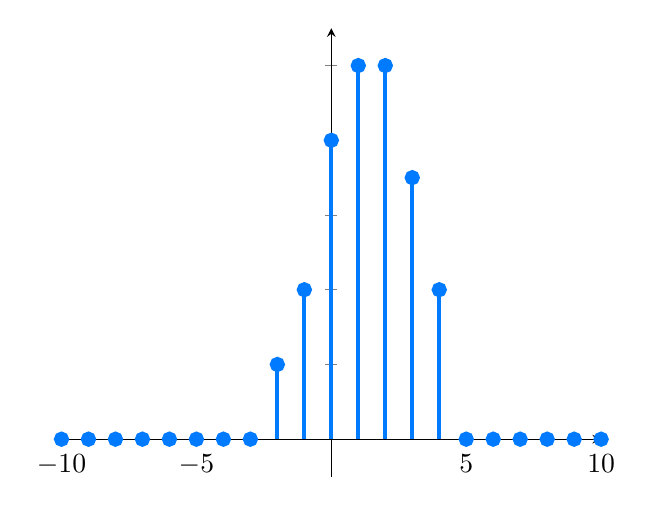
\begin{tikzpicture}
        \begin{axis}[
          xmin= -10, xmax= 10,
          ymin= -0.1, ymax = 1.1,
          axis lines = middle,
          yticklabels={},
        ]
        \addplot[lightblue, line width=1.5, ycomb, mark=*] coordinates {
 (-10, 0.0)
(-9, 0.0)
(-8, 0.0)
(-7, 0.0)
(-6, 0.0)
(-5, 0.0)
(-4, 0.0)
(-3, 0.0)
(-2, 0.2)
(-1, 0.4)
(0, 0.8)
(1, 1.0)
(2, 1.0)
(3, 0.7)
(4, 0.4)
(5, 0.0)
(6, 0.0)
(7, 0.0)
(8, 0.0)
(9, 0.0)
(10, 0.0)       

          };
        \end{axis}
      \end{tikzpicture}
    \end{center}
    \begin{enumerate}[label=\color{red}\textbf{\alph*)}]
      \item  \db{$x[n-3]$} 
      
        \begin{minipage}{0.45\textwidth}
       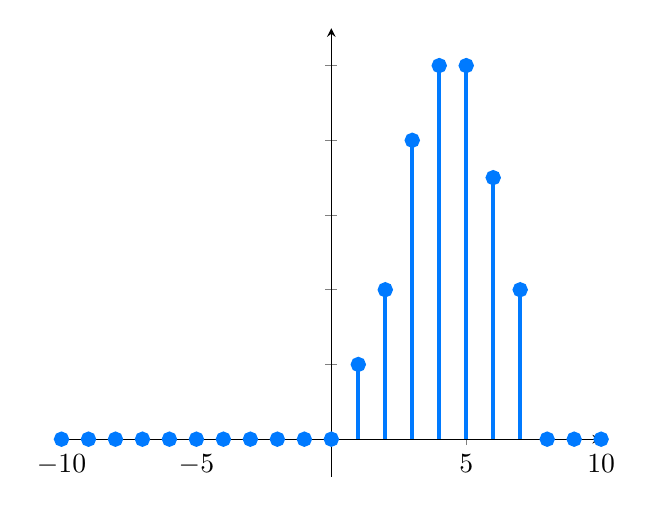
\begin{tikzpicture}
        \begin{axis}[
          xmin= -10, xmax= 10,
          ymin= -0.1, ymax = 1.1,
          axis lines = middle,
          yticklabels={},
        ]
        \addplot[lightblue, line width=1.5, ycomb, mark=*] coordinates {
(-10, 0.0)
(-9, 0.0)
(-8, 0.0)
(-7, 0.0)
(-6, 0.0)
(-5, 0.0)
(-4, 0.0)
(-3, 0.0)
(-2, 0.0)
(-1, 0.0)
(0, 0.0)
(1, 0.2)
(2, 0.4)
(3, 0.8)
(4, 1.0)
(5, 1.0)
(6, 0.7)
(7, 0.4)
(8, 0.0)
(9, 0.0)
(10, 0.0)
          };
        \end{axis}
      \end{tikzpicture}
 
        \end{minipage}\qquad \begin{minipage}{0.45\textwidth}
        Vemos que esta señal se corresponde con un desplazamiento de 3 unidades a la derecha. Por tanto, $x[n-3]=0$ para  $n<1$ y  $n>7$.
        \end{minipage}
      \item \db{$x[n+4]$}
      
 \begin{minipage}{0.45\textwidth}
       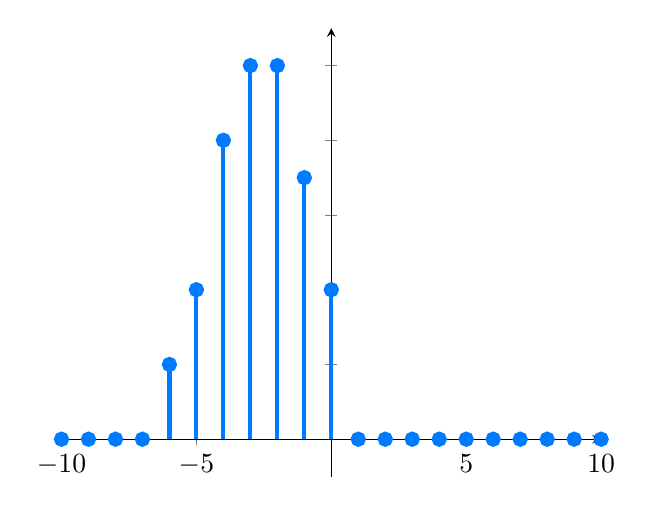
\begin{tikzpicture}
        \begin{axis}[
          xmin= -10, xmax= 10,
          ymin= -0.1, ymax = 1.1,
          axis lines = middle,
          yticklabels={},
        ]
        \addplot[lightblue, line width=1.5, ycomb, mark=*] coordinates {
(-10, 0.0)
(-9, 0.0)
(-8, 0.0)
(-7, 0.0)
(-6, 0.2)
(-5, 0.4)
(-4, 0.8)
(-3, 1.0)
(-2, 1.0)
(-1, 0.7)
(0, 0.4)
(1, 0.0)
(2, 0.0)
(3, 0.0)
(4, 0.0)
(5, 0.0)
(6, 0.0)
(7, 0.0)
(8, 0.0)
(9, 0.0)
(10, 0.0)
          };
        \end{axis}
      \end{tikzpicture}
 
        \end{minipage}\qquad \begin{minipage}{0.45\textwidth}
        Vemos que la señal se corresponde con un desplazamineto de 4 unidades a la izquierda. Por tanto $x[n+4]=0$ para  $n<-6$ y  $n>0$.
        \end{minipage}

      \item \db{$x[-n]$} 
      
 \begin{minipage}{0.45\textwidth}
       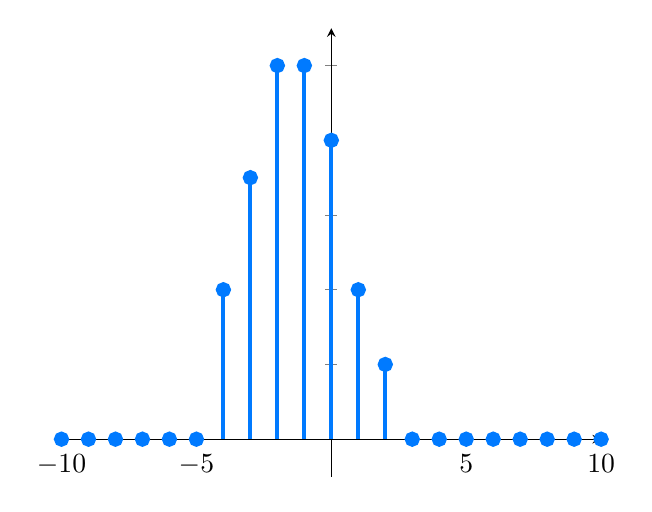
\begin{tikzpicture}
        \begin{axis}[
          xmin= -10, xmax= 10,
          ymin= -0.1, ymax = 1.1,
          axis lines = middle,
          yticklabels={},
        ]
        \addplot[lightblue, line width=1.5, ycomb, mark=*] coordinates {
(-10, 0.0)
(-9, 0.0)
(-8, 0.0)
(-7, 0.0)
(-6, 0.0)
(-5, 0.0)
(-4, 0.4)
(-3, 0.7)
(-2, 1.0)
(-1, 1.0)
(0, 0.8)
(1, 0.4)
(2, 0.2)
(3, 0.0)
(4, 0.0)
(5, 0.0)
(6, 0.0)
(7, 0.0)
(8, 0.0)
(9, 0.0)
(10, 0.0)
          };
        \end{axis}
      \end{tikzpicture}
 
        \end{minipage}\qquad \begin{minipage}{0.45\textwidth}
        Vemos que est señal se corresponde con una reflexión o simetría de la señal con respecto al eje central. Por tanto, $x[-n]=0$ para  $n<-4$ y  $n>2$.
        \end{minipage}

      \item \db{$x[-n+2]$} 

 \begin{minipage}{0.45\textwidth}
       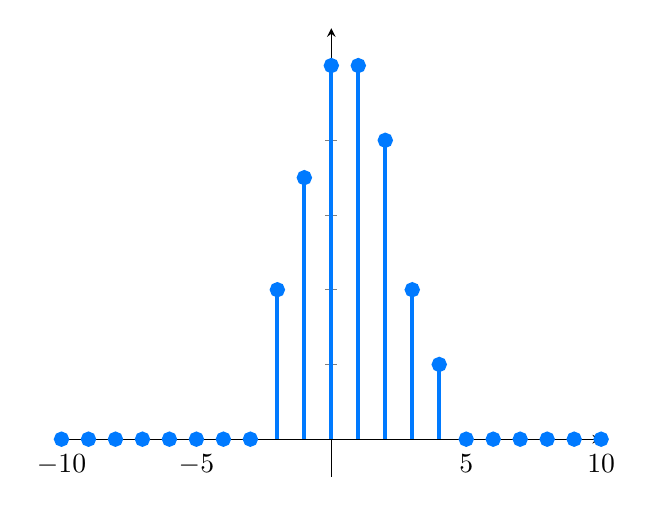
\begin{tikzpicture}
        \begin{axis}[
          xmin= -10, xmax= 10,
          ymin= -0.1, ymax = 1.1,
          axis lines = middle,
          yticklabels={},
        ]
        \addplot[lightblue, line width=1.5, ycomb, mark=*] coordinates {
(-10, 0.0)
(-9, 0.0)
(-8, 0.0)
(-7, 0.0)
(-6, 0.0)
(-5, 0.0)
(-4, 0.0)
(-3, 0.0)
(-2, 0.4)
(-1, 0.7)
(0, 1.0)
(1, 1.0)
(2, 0.8)
(3, 0.4)
(4, 0.2)
(5, 0.0)
(6, 0.0)
(7, 0.0)
(8, 0.0)
(9, 0.0)
(10, 0.0)
          };
        \end{axis}
      \end{tikzpicture}
 
        \end{minipage} \begin{minipage}{0.45\textwidth}
        Vemos que esta señal se corresponde con una reflexión o simetría de la señal con respecto al eje central y un desplazamiento a la derecha de 2 unidades. Por tanto, $x[-n+2]=0$, para  $n<-2$ y  $n>4$
        \end{minipage}

      \item \db{$x[-n-2]$} 

 \begin{minipage}{0.45\textwidth}
       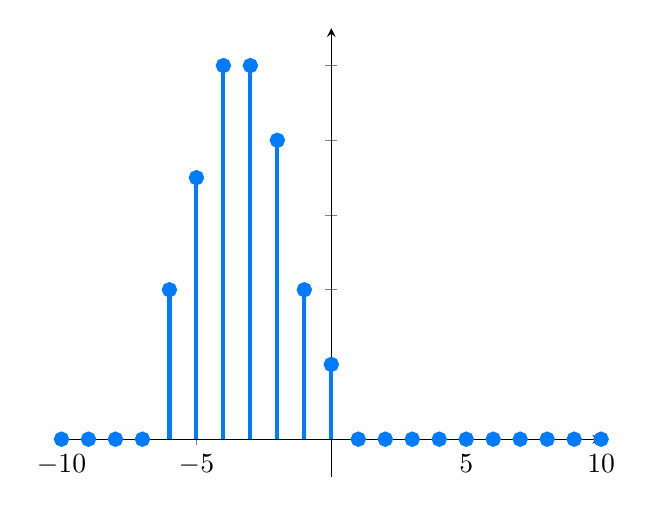
\begin{tikzpicture}
        \begin{axis}[
          xmin= -10, xmax= 10,
          ymin= -0.1, ymax = 1.1,
          axis lines = middle,
          yticklabels={},
        ]
        \addplot[lightblue, line width=1.5, ycomb, mark=*] coordinates {
(-10, 0.0)
(-9, 0.0)
(-8, 0.0)
(-7, 0.0)
(-6, 0.4)
(-5, 0.7)
(-4, 1.0)
(-3, 1.0)
(-2, 0.8)
(-1, 0.4)
(0, 0.2)
(1, 0.0)
(2, 0.0)
(3, 0.0)
(4, 0.0)
(5, 0.0)
(6, 0.0)
(7, 0.0)
(8, 0.0)
(9, 0.0)
(10, 0.0)
          };
        \end{axis}
      \end{tikzpicture}
 
        \end{minipage} \begin{minipage}{0.45\textwidth}
        Vemos que esta señal se corresponde con una reflexión o simetría de la señal con respecto al eje central y un desplazamiento a la izquierda de 2 unidades. Por tanto, $x[-n-2]=0$, para  $n<-6$ y  $n>0$.
        \end{minipage}

    \end{enumerate}
  \item \lb{Considere una señal $x(t)$ en la que  $x(t)=0$ para  $t<3$. Para cada una de las señales siguientes deteremine los valores de $t$ en los que se garantiza que la señal es cero.}
\begin{center}
\includegraphics[width=0.7\linewidth]{"Ejercicio 5/Figure 1"}
\end{center}
    \begin{enumerate}[label=\color{red}\textbf{\alph*)}]
      \item \db{$x(1-t)$} 

\begin{minipage}{0.45\textwidth}
\includegraphics[width=\linewidth]{"Ejercicio 5/Figure 2"}
\end{minipage} \begin{minipage}{0.45\textwidth}
Podemos expresar dicha señal de la forma $x(-t+1)$, donde vemos rápidamente que se trata de una inversión y de un desplazamiento de un segundo hacia la derecha. Por lo tanto, como se muestra en la figura, la señal  $x(1-t)$ será cero para  $t\ge -2$.
\end{minipage}

      \item \db{$x(1-t)+x(2-t)$} 

\begin{minipage}{0.45\textwidth}
\includegraphics[width=\linewidth]{"Ejercicio 5/Figure 3"} 
\end{minipage}\begin{minipage}{0.45\textwidth}
Si la señal $x(1-t)$ es cero para  $t\ge -2$, vemos fácilmente que $x(2-t)$ es cero para  $t\ge -1$. Por lo tanto, al sumarlas, seguirá siendo cero para $t\ge -1$.
\end{minipage}

      \item \db{$x(1-t)x(2-t)$} 
      
      \begin{minipage}{0.45\textwidth}
      \includegraphics[width=\linewidth]{"Ejercicio 5/Figure 4"}
      \end{minipage} \begin{minipage}{0.45\textwidth}
      Si la señal $x(1-t)$ es cero para  $t\ge -2$, vemos fácilmente que $x(2-t)$ es cero para  $t\ge -1$. Por lo tanto, al multiplicarlas, seguirá ´siendo cero para $t\ge -2$.
      \end{minipage}

      \item \db{$x(3t)$} 
      
      \begin{minipage}{0.45\textwidth}
      \includegraphics[width=\linewidth]{"Ejercicio 5/Figure 5"}
      \end{minipage} \begin{minipage}{0.45\textwidth}
      Si la señal $x(t)$ es cero para  $t<3$, al aplicar la compresión por el factor  $a=3$, la señal  $x(3t)$ será cero para  $t>1$.
      \end{minipage}

      \item \db{$x\left( \dfrac{t}{3} \right) $} 

\begin{minipage}{0.45\textwidth}
\includegraphics[width=\linewidth]{"Ejercicio 5/Figure 6"}
\end{minipage} \begin{minipage}{0.45\textwidth}
Si la señal $x(t)$ es cero para  $t<3$, al aplicar la expansión por el factor  $a=\dfrac{1}{3}$, la señal $x\left( \dfrac{t}{3} \right) $ será cero para $t>9$.
\end{minipage}
    \end{enumerate}
  \item \lb{Determine si cada de las siguientes señales es periódica:}
    \begin{enumerate}[label=\color{red}\textbf{\alph*)}]
      \item \db{$x(t)=2e^{j\left( t+\frac{\pi}{4}  \right)u(t) } $} 

        \begin{itemize}[label=\textbullet]
          \item La parte exponencial $\left( e^{j\left( t+\frac{\pi}{4}  \right) }  \right) $ es un señal compleja con una frecuencia $\omega_0=1$, lo cual sugiere periodicidad.
          \item Sin embargo, la función escalón $u(t)$ hace que la señal solo existe para  $t\ge 0$. Esto significa que la señal no se repite en todo el dominio de $t$, por lo tanto, no es periódica.
        \end{itemize}
      \item \db{$x(t)=x[n]=e[n]+u[-n]$} 
        \begin{itemize}[label=\textbullet]
          \item $u[n]$ es la función escalón, que es 1 para  $n\ge 0$ y $0$ para  $n<0$.
          \item  $u[-n]$ es la función escalón reflejada, que es 1 para $n\le 0$ y 0 para $n>0$.
          \item Sumando ambas funciones: la señal es 1 para todo  $n$, es decir,  $x[n]=1$ para todo  $n$, esto hace que la señal sea constante, por lo tanto, es periódica para cualquier período  $N$.
        \end{itemize}
      \item \db{$x[n]=\sum_{k=-\infty}^{\infty} (\delta[n-4k]-\delta[n-1-4k])$}  
        \begin{itemize}[label=\textbullet]
          \item La señal está compuesta por dos deltas desplazadas en el tiempo.
          \item la forma general es de dos impulsos cada intervalo de 4 muestras.
          \item Por lo tanto, la señal es periódica con período $N=4$.
        \end{itemize}
    \end{enumerate}
  \item \lb{Para cada una de las señales siguientes determine los valores de la variable independiente en los que se garantice que la parte par de la señal es cero.}
    \begin{enumerate}[label=\color{red}\textbf{\alph*)}]
      \item \db{$x[n]=u[n]-u[n-4]$} 

        Esta señal es un tren de impulsos rectangular con valores de 1, en $0\le n\le 3$ y 0 en otros lugares.
        \begin{itemize}[label=\textbullet]
          \item Antisimetría respecto a $n=\dfrac{3}{2}$, por lo que su parte par será cero en los puntos donde $x[n]=-x[-n]$.
          \item Para $n=0,1,2,3$ tenemos valores de 1.
          \item Para  $n=-1,-2,-3$, la función es 0.
          \item La parte par será cero en los valores fuera del intervalo  $[-3,3]$.
        \end{itemize}
      \item $\db{x(t)=\sin\left( \dfrac{t}{2} \right) } $ 

        La función seno es impar, es decir: \[
        \sin\left( \dfrac{t}{2} \right) +\sin\left( \dfrac{t}{2} \right) =0
        \] 
        Por definición, su parte par es cero para todo $t$.
      \item \db{$x[n]=\left( \dfrac{1}{2} \right) ^nu[n-3]$}

        Esta señal es una secuencia geométrica desplazada a partir de $n=3$, es decir:  \[
          x[n]=\begin{cases}
            \left( \dfrac{1}{2} \right) ^{n} & \text{si }n\ge 3\\
            0 & \text{en otro caso}
          \end{cases}
        \] 
        Para que su parte par sea cero, debe cumplirse $x[n]=-x[-n]$, pero como la función es unilateral, su parte par será cero donde  $x[n]=0$, es decir, donde  $n<3$.
      \item \db{$x(t)=e^{-5t}u(t+2) $} 

        Esta señal es una exponencial decreciente activada en $t\ge -2$.
        \begin{itemize}[label=\textbullet]
          \item Es unilateral y no tiene valores negativos simétricos, por lo que su parte par será cero antes de la activación, es decir, cuando $t\le -2$.
        \end{itemize}
    \end{enumerate}
  \item \lb{Exprese la parte real de cada una de las siguientes señales de la forma $Ae^{-at}\cos(\omega t+\varphi) $, donde $A,a,\omega$ y $\varphi$ son números reales con $A\ge 0$ y $-\pi\le \varphi\le \pi$.} 
    \begin{enumerate}[label=\color{red}\textbf{\alph*)}]
      \item \db{$x(t)=-2$} 
        \[
        x(t)=2e^{-0t}\cos(0t+\pi), 
        \] donde: \[
        \begin{array}{ll}
          \bullet\, A=2 & \bullet\, \omega=0\\
          \bullet\, a=0 & \bullet\, \varphi=\pi
        \end{array}
        \] 
      \item \db{$x(t)=\sqrt{2} e^{j\frac{\pi}{4} } \cos(3t+2\pi)$} 

        $x(t)=\sqrt{2} e^{j\frac{\pi}{4} } \cos(\lbb{3t+2\pi}{\theta+2\pi=\theta})=\sqrt{2}\left( \cos\left( \dfrac{\pi}{4} \right) +j\cdot \sin\left( \dfrac{\pi}{4} \right)  \right) \cos(3t)=(1+j)\cos(3t)$

        Solo tomamos la parte real, por lo que: \[
        x(t)=\cos\left( 3t+\dfrac{\pi}{4} \right) ,
        \] donde: \[
        \begin{array}{ll}
          \bullet\, A=1 & \bullet\, \omega=3\\
          \bullet\, a=0 & \bullet\,\varphi=\dfrac{\pi}{4}
        \end{array}
        \] 
      \item \db{$x(t)=e^{-t}\sin(3t+\pi) $} 

        Usaremos la identidad: \[
        \sin(\theta)=\cos\left( \theta-\dfrac{\pi}{2} \right) ,
        \] por lo que: \[
        x(t)=e^{-t}\cos\left( 3t+\pi-\dfrac{\pi}{2} \right) =e^{-t}\cos\left( 3t+\dfrac{\pi}{2} \right)   ,
        \] donde: \[
        \begin{array}{ll}
          \bullet\, A=1 & \bullet\,\omega=3\\
          \bullet\, a=1 & \bullet\, \varphi=\dfrac{\pi}{2}
        \end{array}
        \] 
      \item \db{$x(t)=je^{(-2+j 100)t} $} 
    \end{enumerate}
  \item \lb{Determine si cada una de las siguientes señales es periódica. En caso afirmativo especifique su periodo fundamental.}
    \begin{enumerate}[label=\color{red}\textbf{\alph*)}]
      \item \db{$x(t)=-2$} 

        La señal tiene la forma $x(t)=e^{j\omega t} $, que es periódica si la frecuencia angular $\omega$ es un múltiplo racional de $2\pi$: \[
        \omega=10.
        \] 
        El periodo fundamental es: \[
        T=\dfrac{2\pi}{\omega}=\dfrac{2\pi}{10}=\dfrac{\pi}{5}.
        \] 
        La señal es periódica con periodo fundamental $T=\dfrac{\pi}{5}$.
      \item \db{$x(t)=e^{(-1+j)t} $} 

        Esta señal tiene un término $e^{-t} $, que representa un decrecimiento exponencial. Si hay un término exponencial con un exponente real negativo, la señal nunca se repite exactamente, ya que disminuye continuamente, por lo tanto, no es periódica.
      \item \db{$x[n]=e^{j 7\pi n} $} 

        $\omega=7\pi\longrightarrow N=\dfrac{2\pi}{\omega}\cdot m=\dfrac{2\pi}{7\pi}\cdot m=\dfrac{2}{7}\cdot m\longrightarrow N=2\:(m=7)$

        La señal es periódica, con periodo fundamental $N=2$.
      \item \db{$x[n]=3e^{j3\pi\frac{n+\frac{1}{2} }{5} } $} 

        $\omega=\dfrac{2\pi}{5}\longrightarrow N=\dfrac{2\pi}{\omega}\cdot m=\dfrac{2\pi}{\frac{3\pi}{5} }\cdot m=\dfrac{10}{3}\cdot m\longrightarrow N=10\:(m=3)$
      \item \db{$x[n]=3e^{j\frac{3}{5} \left( n+\frac{1}{2}  \right) } $} 

        $\omega=\dfrac{3}{5}\longrightarrow N=\dfrac{2\pi}{\omega}\cdot m=\dfrac{2\pi}{\frac{3}{5} }\cdot m=\dfrac{10\pi}{3}\cdot m\longrightarrow $ No se puede.

        La señal no es periódica.
    \end{enumerate}
  \item \lb{Determine el periodo fundamental de la señal $x(t)=2\cos(10t+1)-\sin(4t-1)$.} 

        Para determinar el \textbf{periodo fundamental} de la señal $x(t)=2\cos(10t+1)-\sin(4t-1)$, debemos analizar los periodos de las componentes individuales de la señal y encontrar el \textbf{mínimo común múltiplo} de estos periodos.
        \begin{enumerate}[label=Paso \arabic*:]
            \item Identificar las frecuencias angulares

                La señal está compuesta por dos términos:
                \begin{itemize}[label=\textbullet]
                    \item $2\cos(10t+1)$: Su frecuencia angular es $\omega_1=10$.
                    \item $-\sin(4t-1)$: Su frecuencia angular es $\omega_2=4$.
                \end{itemize}
                El periodo de una señal está relacionado con su frecuencia angular mediante la fórmula: \[
                T=\dfrac{2\pi}{\omega}.
                \] 
            \item Calcular los periodos de las componentes
                \begin{itemize}[label=\textbullet]
                    \item Para $\omega_1=10$, el periodo es: \[
                    R=\dfrac{2\pi}{10}=\dfrac{\pi}{5}.
                    \] 
                \item Para $\omega_2=4$, el periodo es: \[
                T_2=\dfrac{2\pi}{4}=\dfrac{\pi}{2}.
                \] 
                \end{itemize}
            \item Encontrar el periodo fundamental

                El periodo fundamental de la señal compuesta es el \textbf{mínimo común múltiplo} de los periodos $T_1$ y $T_2$. Para encontrarlo, debemos expresar ambos periodos como fracciones con el mismo denominador: \[
                T_1=\dfrac{\pi}{5},\quad T_2=\dfrac{\pi}{2}\longrightarrow T_1=\dfrac{2\pi}{10},\quad T_2=\dfrac{5\pi}{10}\longrightarrow .
                \]  
                El \textbf{mcm} de $\dfrac{2\pi}{10}$ y $\dfrac{5\pi}{10}$ es $\dfrac{10\pi}{10}=\pi$.
        \end{enumerate}
        El periodo fundamental de la señal $x(t)$ es:  \[
        T=\pi.
        \] 
  \item \lb{Determine el periodo fundamental de la señal $x[n]=1+e^{j\frac{4\pi n}{7}}-e^{j\frac{2\pi n}{5} }$.}
  \item \lb{Considere la señal en tiempo discreto $x[n]=1-\sum_{k=3}^{\infty} \delta[n-1-k]$. Determine los valores de los números enteros $M$ y  $n_0$ que permiten que $x[n]$ pueda expresarse como  $x[n]=u[Mn+n_0]$} 
  \item \lb{Considere la señal en tiempo continuo $x(t)=\delta(t+2)-\delta(t+2)$. Calcule la energía de la señal  $y(t)=\int_{-\infty}^{t} x(\tau)\mathrm{d}\tau $.}
  \item \lb{La figura 1 muestra la señal continua $x(t)$. Represente cada una de las siguientes señales.}
    \begin{center}
      \begin{tikzpicture}[scale=1.5]
        \draw (-2.5,0) -- (2.5,0) node[right] {$t$};
        \draw (0,-1.5) -- (0,2.5) node[above] {$x(t)$};
        \draw[lightblue, line width=1.5] (-2, 0) -- (-2,-1) -- (-1,0) -- (-1, 1) -- (0,1) -- (0,2) -- (1,2) -- (1,1) -- (2,0);
        \foreach \x in {-2,...,2} {\node[below] at (\x,0) {$\x$};}
        \foreach \y in {-1, 1} {\node[right] at (0,\y) {$\y$};}
        \node[left] at (0,2) {$2$};
      \end{tikzpicture}\\
      \lb{Figura 1} 
    \end{center}
    \begin{enumerate}[label=\color{red}\textbf{\alph*)}]
      \item \db{$x(t-1)$} 
      \item \db{$x(2-t)$} 
      \item \db{$x(2t+1)$} 
      \item \db{$x\left( 4-\dfrac{t}{2} \right) $} 
      \item \db{$[x(t)+x(-t)]u(t)$} 
      \item \db{$x(t)\left[ \delta\left( t+\dfrac{3}{2} \right) -\delta\left( t-\dfrac{3}{2} \right)  \right] $} 
    \end{enumerate}
  \item \lb{La figura 2 muestra la señal discreta $x[n]$. Represente cada una de las siguientes señales:}
    \begin{center}
      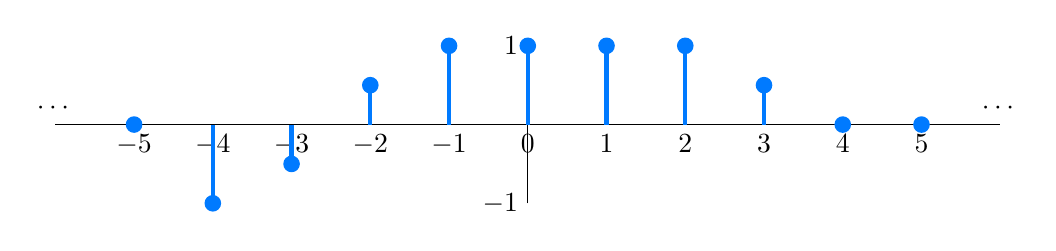
\begin{tikzpicture}
        \draw (-6,0) node[above] {$\cdots$} -- (6,0) node[above] {$\cdots$};
        \draw (0,-1) node[left] {$-1$} -- (0,1) node[left] {$1$};
        \foreach \x/\y in {-5/0,-4/-1,-3/-0.5,-2/0.5, -1/1, 0/1, 1/1, 2/1, 3/0.5, 4/0, 5/0} {
        \node[below] at (\x,0) {$\x$};
        \draw[lightblue, line width=1.5] (\x,0) -- (\x,\y);
        \fill[lightblue] (\x,\y) circle (3pt);
        }
      \end{tikzpicture}\\
      \lb{Figura 2} 
    \end{center}
    \begin{enumerate}[label=\color{red}\textbf{\alph*)}]
      \item \db{$x[n-4]$} 
      \item \db{$x[3-n]$} 
      \item \db{$x[3n]$} 
      \item \db{$x[3n+1]$} 
      \item \db{$x[n]u[3-n]$} 
      \item \db{$x[n-3]\delta[n-2]$} 
      \item \db{$\dfrac{1}{2}x[n]+\dfrac{1}{2}(-1)^nx[n]$} 
      \item \db{$x[(n-1)^2]$} 
    \end{enumerate}
  \item \lb{Determine si cada una de las siguientes señales continuas es periódica. En caso afirmativo obtenga su periodo fundamental.}
    \begin{enumerate}[label=\color{red}\textbf{\alph*)}]
      \item \db{$x(t)=3\cos\left(4t+\dfrac{\pi}{3}\right)$} 
      \item \db{$x(t)=e^{j(\pi t-1)} $} 
      \item \db{$x(t)=\cos^2\left( 2t-\dfrac{\pi}{3} \right) $} 
      \item \db{$x(t)=\mathrm{Par}\{\cos(4\pi t)u(t)\} $} 
      \item \db{$x(t)=\mathrm{Par}\{\sin(4\pi t)u(t)\} $} 
      \item \db{$x(t)=\sum_{n=-\infty}^{\infty} e^{-(2t-n)}u(2t-n) $} 
    \end{enumerate}
\end{enumerate}
\end{document}
